%@TheDoctorRAB
%
%presentation template for class slides and research presentations
%allows for citations in slide and a list at the end
%
%%%%%
%
%REFERENCES
%
%neup.bst - numbered citations in order of appearance, short author list with et al in reference section
%nsf.bst - numbered citations in order of appearance, full author list in references section
%standard.bst - citations with author last name with et al for more than 2 authors; full author list in references section
%ans.bst is for ANS only. 
%
%author = {Lastname, Firstname and Lastname, Firstname and Lastname, Firstname} for all bst formats
%bst renders the author list itself
%
%author = {{Nuclear Regulatory Commission}} if the author is an organization, institution, etc., and not people
%
%title = {{}} for all
%
%for all - use \citep{-} - [1] or (Borrelli, 2021) in the text
%standard.bst \cite{-} - Borrelli (2021) in the text
%standard.bst lists references alphabetically
%the rest list numerically
%
%
%%% citations on slides 
%
%\citep{xxxnna} where the citation should go
%\blfootnote{\fontsize\cite{xxxnna}\fontsize\bibentry{xxxnna}} before \end{frame}
%
%
%%%%%

%%%%% presentation settings
\documentclass[aspectratio=1610,pdftex,dvipsnames,compress,xcolor={dvipsnames}]{beamer}
\usetheme{Boadilla}
\usecolortheme{seahorse}
\beamertemplatenavigationsymbolsempty
\addtobeamertemplate{footnote}{\hskip -2em}{} %pushes footnote to margin
%%% font style - can add size, etc.
%https://tug.ctan.org/macros/latex/contrib/beamer/doc/beameruserguide.pdf
\setbeamerfont{title}{series=\bfseries}
\setbeamerfont{frametitle}{series=\bfseries}
\setbeamerfont{footline}{series=\bfseries}
\setbeamerfont{author}{series=\bfseries}
\setbeamerfont{institute}{series=\bfseries}
\setbeamerfont{date}{series=\bfseries}
\setbeamertemplate{page number in head/foot}[framenumber] %just gives slide number; comment out for 1/7, 2/7...
%%%%%


%%%%% colors
%http://latexcolor.com/
%https://en.wikibooks.org/wiki/LaTeX/Colors#:~:text=black%2C%20blue%2C%20brown%2C%20cyan,be%20available%20on%20all%20systems.
%sam root
\definecolor{BackGround}{RGB}{255,250,240}
\definecolor{PrideGold}{RGB}{241,179,0}
\definecolor{Silver}{RGB}{165,169,180}
\definecolor{White}{RGB}{255,255,255}
\definecolor{Black}{RGB}{25,25,25}
\definecolor{Chrome}{RGB}{245,245,245}
%%% general
\definecolor{aliceblue}{rgb}{0.94, 0.97, 1.0}
\definecolor{antiquewhite}{rgb}{0.98, 0.92, 0.84}
\definecolor{lightmauve}{rgb}{0.86, 0.82, 1.0}
\definecolor{brilliantlavender}{rgb}{0.96, 0.73, 1.0}
\definecolor{brandeisblue}{rgb}{0.0, 0.44, 1.0}
\definecolor{darkmidnightblue}{rgb}{0.0, 0.2, 0.4}
\definecolor{darkchampagne}{rgb}{0.76, 0.7, 0.5}
%%% set slides
\setbeamercolor{background canvas}{bg=BackGround}
%%%
\setbeamercolor{block title}{bg=Silver,fg=Black}
\setbeamercolor{block body}{bg=Silver!20,fg=Black}
\setbeamercolor{block title alerted}{bg=Black,fg=Silver}
\setbeamercolor{block body alerted}{bg=PrideGold,fg=Black}
\setbeamercolor{alerted text}{fg=Silver}
\setbeamercolor*{block title example}{bg=PrideGold,fg=Black}
\setbeamercolor*{block body example}{bg=PrideGold!20,fg=Black}
%%%
\setbeamercolor*{palette primary}{bg=PrideGold,fg=Black}
\setbeamercolor*{palette secondary}{bg=PrideGold,fg=Black}
\setbeamercolor*{palette tertiary}{bg=PrideGold,fg=Black}
%%%
\setbeamercolor*{titlelike}{bg=PrideGold,fg=Black}
\setbeamercolor*{title}{bg=PrideGold,fg=Black}
\setbeamercolor*{item}{fg=PrideGold}
\setbeamercolor*{caption name}{fg=PrideGold}
%%%
\setbeamercolor*{sidebar}{fg=PrideGold,bg=Black}
\setbeamercolor*{title in sidebar}{fg=PrideGold}
\setbeamercolor*{author in sidebar}{fg=PrideGold}
\setbeamercolor*{section in sidebar}{fg=PrideGold}
%%%
\setbeamercolor{section in toc}{fg=Black}
\setbeamercolor{subsection in toc}{fg=Black}
%%%
\setbeamercolor{page number in head/foot}{fg=Black,bg=PrideGold}
%\setbeamercolor{footline}{bg=Black}
%%%
\setbeamercolor{bibliography entry author}{fg=Black}
\setbeamercolor{bibliography entry note}{fg=Black}
\setbeamercolor{bibliography entry title}{fg=Black}
%%%
\newcommand{\x}{\cellcolor{aliceblue}} %use to shade in table cell
\newcommand{\y}{\cellcolor{lightgray}} %use to shade in table cell
\newcommand{\z}{\cellcolor{antiquewhite}} %use to shade in table cell
\newcommand{\w}{\cellcolor{darkchampagne}} %use to shade in table cell

%%%%%


%%%%% general 
%\documentclass[11pt,a4paper]{article}
%\usepackage[lmargin=1in,rmargin=1in,tmargin=1in,bmargin=1in]{geometry}
\usepackage[pagewise]{lineno} %line numbering
\usepackage{setspace}
\usepackage{ulem} %strikethrough - do not \sout{\cite{}}
\usepackage{graphicx}
\usepackage{mypythonhighlight,verbatim}
\usepackage{filecontents}
\usepackage{tablefootnote}
\usepackage{footnotehyper}
\usepackage{float}
%\usepackage{subfig}
\usepackage[yyyymmdd]{datetime} %date format
\renewcommand{\dateseparator}{.}
\graphicspath{{$TEXIMG/}} %path to graphics
\setcounter{secnumdepth}{5} %set subsection to nth level
\usepackage{needspace}
\usepackage[stable,hang,flushmargin]{footmisc} %footnotes in section titles and no indent; standard.bst
\usepackage[inline]{enumitem}
\setlist[itemize]{label=\textbullet}
\usepackage{boldline}
\usepackage{makecell}
\usepackage{booktabs}
\usepackage{amssymb}
\usepackage{gensymb}
\usepackage{amsmath,nicefrac}
\usepackage{physics}
\usepackage{lscape}
\usepackage{array}
\usepackage{chngcntr}
\usepackage{hyperref}
\hypersetup{colorlinks,linkcolor=black,citecolor=black,urlcolor=blue} 
%\usepackage{sectsty}
\usepackage{textcomp}
\usepackage{lastpage}
\usepackage{xargs} %for \newcommandx
\usepackage[colorinlistoftodos,prependcaption,textsize=tiny]{todonotes} %makes colored boxes for commenting
\usepackage{soul}
\usepackage{color}
\usepackage{marginnote}
\usepackage[figure,table]{totalcount}
\usepackage[capitalise]{cleveref}
\usepackage{microtype} %improves typography for pdf
\usepackage[pdftex,dvipsnames]{colortbl} %change font color
%%%%%


%%%%% tikz
\usepackage{pgf}
\usepackage{tikz} % required for drawing custom shapes
\usetikzlibrary{shapes,arrows,automata,trees}
%%%%%


%%%%% fonts
\usepackage{times}
%\renewcommand{\sfdefault}{ubuntu}
%arial - uncomment next two lines
%\usepackage{helvet}
%\renewcommand{\familydefault}{\sfdefault}
%%%%%


%%%%% references
%\usepackage[round,semicolon]{natbib} %for (Borrelli 2021; Clooney 2019) - standard.bst 
\usepackage[numbers,sort&compress]{natbib} %for [1-3] - nsf.bst, neup.bst
\usepackage{bibentry}
\setlength{\bibsep}{7pt} %sets space between references
%\renewcommand{\bibsection}{} %suppresses large 'references' heading
%\renewcommand\bibpreamble{\vspace{\baselineskip}} %sets spacing after heading if not using default references heading
%%%%%


%%%%% tables and figures
\usepackage{longtable} %need to put label at top under caption then \\ - use spacing
\usepackage{makecell}
\usepackage{tablefootnote}
\usepackage{tabularx}
\usepackage{multirow}
\usepackage{tabto} %general tabbed spacing
\usepackage{pdfpages}
\usepackage{wrapfig} %wraps figures around text
\setlength{\intextsep}{0.00mm}
\setlength{\columnsep}{1.00mm}
\usepackage[singlelinecheck=false,labelfont=bf]{caption}
\usepackage{subcaption}
\captionsetup[table]{justification=justified,skip=5pt,labelformat={default},labelsep=period,name={Table}} %sets a space after table caption
\captionsetup[figure]{justification=justified,skip=5pt,labelformat={default},labelsep=period,name={Figure}} %sets space above caption, 'figure' format
\captionsetup[wrapfigure]{justification=centering,aboveskip=0pt,belowskip=0pt,labelformat={default},labelsep=period,name={Fig.}} %sets space above caption, 'figure' format
\captionsetup[wraptable]{justification=centering,aboveskip=0pt,belowskip=0pt,labelformat={default},labelsep=period,name={Table}} %sets space above caption, 'figure' format
%%%%%


%%%%% watermark
%\usepackage[firstpage,vpos=0.63\paperheight]{draftwatermark}
%\SetWatermarkText{\shortstack{DRAFT\\do not distribute}}
%\SetWatermarkScale{0.20}
%%%%%


%%%%% cross referencing files
%\usepackage{xr} %for revisions - will cross reference from one file to here
%\externaldocument{/path/to/auxfilename} %aux file needed
%%%%%


%%%%% toc and glossaries
\usepackage[toc,title]{appendix}
\usepackage[acronym,nomain,nonumberlist]{glossaries}
%\makenoidxglossaries
%\usepackage{titlesec,titletoc}
%\renewcommand{\thepart}{ARTICLE \Roman{part}} %puts the label into the command so \thelabel will carry through
%\renewcommand{\thesection}{\arabic{section}} %puts the label into the command so \thelabel will carry through
%\titleformat{\part}{\normalfont\large\bfseries}{\thepart}{}{}[]
%\titlespacing*\part{0pt}{0.95\baselineskip}{0.75\baselineskip}
%\titleformat{\section}[runin]{\normalfont\large\bfseries}{\thesection}{-1em}{}[.]
%\titlespacing*\section{0pt}{0.65\baselineskip}{0.55\baselineskip}
%\titleformat{\subsection}[runin]{\normalfont\normalsize\bfseries}{\thesubsection}{-1em}{}[.]
%\titlespacing*\subsection{0pt}{0.50\baselineskip}{0.35\baselineskip}
%\titleformat{\paragraph}[runin]{\normalfont\normalsize\bfseries\itshape}{\theparagraph}{-1em}{}[.]
%\titlespacing*\paragraph{0pt}{0.45\baselineskip}{0.25\baselineskip}
%\titleformat{\subparagraph}[runin]{\normalfont\normalsize\itshape}{\thesubparagraph}{-1em}{}[.]
%\titlespacing*\subparagraph{0pt}{0.40\baselineskip}{0.25\baselineskip}
%\titleformat{\paragraph}[hang]{\normalfont\normalsize\bfseries}{\theparagraph}{5pt}{}[]
%\titlespacing*\paragraph{0pt}{0.50\baselineskip}{0.25\baselineskip}
%\titleformat{\subparagraph}[runin]{\normalfont\normalsize\itshape}{\thesubparagraph}{-1em}{}[.]
%\titlespacing*\subparagraph{0pt}{0.40\baselineskip}{0.20\baselineskip}
%%%%%


%%%%% editing
\newcommand{\edit}[1]{\textcolor{blue}{#1}} %shortcut for changing font color on revised text
\newcommand{\fn}[1]{\footnote{#1}} %shortcut for footnote tag
\newcommand*\sq{\mathbin{\vcenter{\hbox{\rule{.3ex}{.3ex}}}}} %makes a small square as a separator $\sq$
%\newcommand{\sk}[1]{\sout{#1}} %shortcut for default strikethrough - do not sk through citep
\newcommand\sk{\bgroup\markoverwith{\textcolor{red}{\rule[0.5ex]{1pt}{1pt}}}\ULon} %strikethrough with red line; not in \section{}
%\st{} does strikethrough using soul package but does not like acronyms
\newcommand{\blucell}{\cellcolor{aliceblue}} %use to shade in table cell
\newcommand{\grycekk}{\cellcolor{lightgray}} %use to shade in table cell
\newcommand{\whicell}{\cellcolor{antiquewhite}} %use to shade in table cell
%%%%%


%%%%% acronyms
\newcommand{\acf}{\acrfull} %full acronym
\newcommand{\acl}{\acrlong} %long acronym
\newcommand{\acs}{\acrshort} %short acronym

\newcommand{\acfp}{\acrfullpl} %full acronym plural
\newcommand{\aclp}{\acrlongpl} %long acronym plural
\newcommand{\acsp}{\acrshortpl} %short acronym plural
%%%%%


%%%%% todonotes
\newcommandx{\cmt}[2][1=]{\todo[author=\textbf{STRUCTURE},tickmarkheight=0.15cm,linecolor=red,backgroundcolor=red!25,bordercolor=black,#1]{#2}}
\newcommandx{\con}[2][1=]{\todo[author=\textbf{CONTENT},tickmarkheight=0.15cm,linecolor=brilliantlavender,backgroundcolor=brilliantlavender,bordercolor=black,#1]{#2}}
%\newcommandx{\rab}[2][1=]{\todo[noline,author=\textbf{RAB},backgroundcolor=Plum!25,bordercolor=black,#1]{#2}}
%%%
%\newcommandx{\jon}[2][1=]{\todo[noline,author=\textbf{ATTN: Johnson},backgroundcolor=blue!25,bordercolor=black,#1]{#2}}
%\newcommandx{\han}[2][1=]{\todo[noline,author=\textbf{ATTN: Haney},backgroundcolor=OliveGreen!25,bordercolor=black,#1]{#2}}
\newcommandx{\rab}[2][1=]{\todo[author=\textbf{Borrelli},tickmarkheight=0.15cm,linecolor=black,backgroundcolor=Plum!25,bordercolor=black,#1]{#2}}
%\newcommandx{\han}[2][1=]{\todo[author=\textbf{ATTN: Haney},tickmarkheight=0.15cm,linecolor=OliveGreen,backgroundcolor=OliveGreen!25,bordercolor=OliveGreen,#1]{#2}}
%\newcommandx{\jon}[2][1=]{\todo[author=\textbf{ATTN: Johnson},tickmarkheight=0.15cm,linecolor=blue,backgroundcolor=blue!25,bordercolor=blue,#1]{#2}}
%%% highlighting 
\DeclareRobustCommand{\hlc}[1]{{\sethlcolor{LimeGreen}\hl{#1}}}
\makeatletter
    \if@todonotes@disabled
    \newcommand{\hlh}[2]{#1}
    \else
    \newcommand{\hlh}[2]{\han{#2}\hlc{#1}}
    \fi
    \makeatother

\DeclareRobustCommand{\hld}[1]{{\sethlcolor{CornflowerBlue}\hl{#1}}}
\makeatletter
    \if@todonotes@disabled
    \newcommand{\hlj}[2]{#1}
    \else
    \newcommand{\hlj}[2]{\jon{#2}\hld{#1}}
    \fi
    \makeatother

\DeclareRobustCommand{\hlf}[1]{{\sethlcolor{lightmauve}\hl{#1}}}
\makeatletter
    \if@todonotes@disabled
    \newcommand{\hlb}[2]{#1}
    \else
    \newcommand{\hlb}[2]{\rab{#2}\hlf{#1}}
    \fi
    \makeatother
%%%%%


%%%%% table alignments
\newcolumntype{L}[1]{>{\raggedright\let\newline\\\arraybackslash\hspace{0pt}}m{#1}} %uses \raggedright with m,p{} in table column
\newcolumntype{C}[1]{>{\centering\let\newline\\\arraybackslash\hspace{0pt}}m{#1}} %uses \raggedright with m,p{} in table column
\newcolumntype{R}[1]{>{\raggedleft\let\newline\\\arraybackslash\hspace{0pt}}m{#1}} %uses \raggedright with m,p{} in table column
%%%%%


%%%%% table contents
\makeatletter
\renewcommand\tableofcontents{%
    \@starttoc{toc}%
}
\makeatother

\makeatletter
\renewcommand\listoffigures{%
    \@starttoc{lof}%
}
\makeatother

\makeatletter
\renewcommand\listoftables{%
    \@starttoc{lot}%
}
\makeatother

\makeatletter
\newcommand*\ftp{\fontsize{16.5}{17.5}\selectfont}
\makeatother
%%%%%


%%%%% user commands
\newcommand\blfootnote[1]{%
  \begingroup
  \renewcommand\thefootnote{}\footnote{#1}%
  \addtocounter{footnote}{-1}%
  \endgroup
}


\makeatletter
\renewcommand{\@biblabel}[1]{#1.\hfill} %bibliography ordered list has numbers left flush
\makeatother


\AtBeginSection[]{
    \begin{frame}[plain]{}
         
         \vfill

         \centering
         \begin{beamercolorbox}[sep=8pt,center,shadow=true,rounded=true]{titlelike}
             \usebeamerfont{title}\insertsectionhead\par
         \end{beamercolorbox}

         \vfill

     \end{frame}
 }
%%%%%


%%%%% header and footer
%\usepackage{fancyhdr}
%\pagestyle{fancy}
%\fancyhf{} %move page number to bottom right
%\renewcommand{\headrulewidth}{0pt} %set line thickness in header; uncomment as is to remove line
%\lhead{\scriptsize Name}
%\lhead{\scriptsize PNUCENE-D-22-xxxxx}
%\chead{\scriptsize \textit{PhD White Paper Project Proposal}}
%\rhead{\scriptsize \today}
%\rfoot{\thepage}
%%%%%


%%%%% acronyms
\input{$ACRONYM/acronyms}
%%%%%

%%%%% spacing
%\onehalfspacing %linespacing
%\setstretch{1.05} %linespacing
%\spacing{1.25} %equivalent to 1.5 line spacing in Word
%%%%%


%%%%% linenumbering
%\linenumbers %toggle line numbers
%\pagewiselinenumbers %reset line numbers on new page
%\modulolinenumbers[1] %line numbering interval
%%%%%


%%%%% title page
\addtocounter{framenumber}{-1} %does not count the title slide in the slide count
\title[NE585 - Nuclear fuel cycles]{NE585\\NUCLEAR FUEL CYCLES\\Nuclear engineering basics\\1}
\author[@TheDoctorRAB]{R. A. Borrelli}
\institute[]{
    \acl{ui}\\
    \vspace{0.10in}
    
\includegraphics[width=0.20\textwidth]{logo/university-of-idaho/nuclear-engineering/ne-logo.png}
    }
\date{\acl{iff}}
%%%%%


\begin{document}


%%%%% title page with no footer
{
    \setbeamertemplate{footline}{}
    \begin{frame}
        \titlepage
    \end{frame}
}
%%%%%


\begin{frame}{Learning objectives}
    \begin{enumerate}[series=outerlist,topsep=0pt,itemsep=21pt,leftmargin=*,label=(\arabic*)]
        \item[]Demonstrating fundamental concepts in nuclear physics
        \item[]Analyzing decay data to identify radionuclides
        \item[]Summarizing different decay mechanisms
        \item[]Book -- Chapter 2
    \end{enumerate}
\end{frame}


\begin{frame}{Learning nodes}
            \begin{enumerate}[series=outerlist,topsep=0pt,itemsep=18pt,leftmargin=*,label=(\arabic*)]
                \item[]\textbf{Relativity}
                \item[]\textbf{Atomic structure}
                \item[]\textbf{Binding energy}
                \item[]\textbf{Q-value}
                \item[]\textbf{Radioactivity}
                \item[]\textbf{Chart of the nuclides}
                \item[]\textbf{Decay chains}
                \item[]\textbf{Half life}
            \end{enumerate}
\end{frame}


\begin{frame}{}
    \begin{figure}
        \centering
        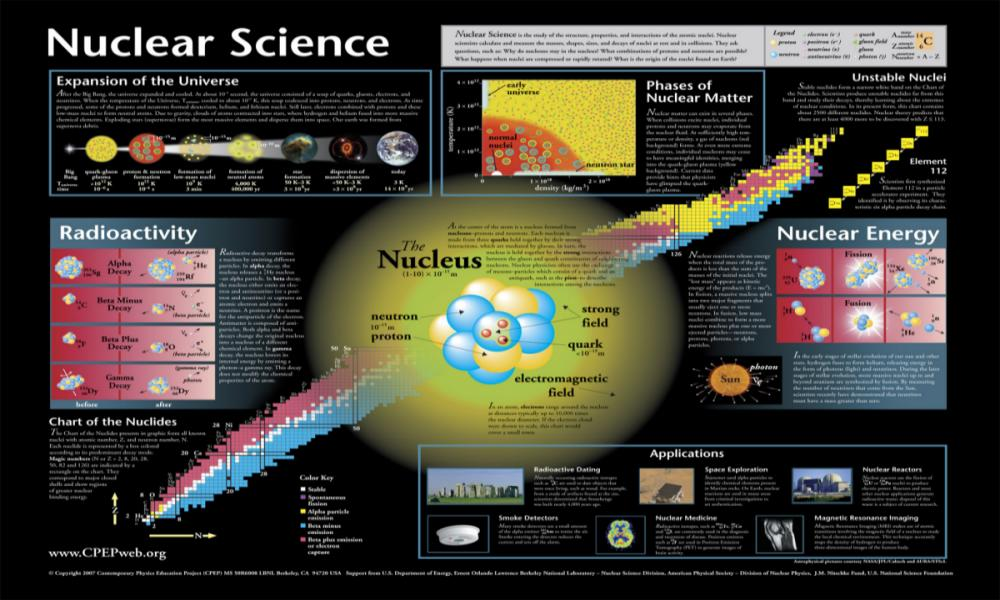
\includegraphics[width=0.95\textwidth]{ne585/nuclear.infographic.jpg}
%        \caption{}
    \end{figure}
\end{frame}


\section{Relativity}


\addtocounter{framenumber}{-1}
\begin{frame}{We apply energy from nuclear reactions and radiation interactions with matter}
    \begin{equation}
        \LARGE
        E_{REST} = m_0 c^2
    \end{equation}

    \begin{equation}
        \LARGE
        E = m c^2
    \end{equation}

    \vspace*{\fill}

    \begin{enumerate}[series=outerlist,topsep=0pt,itemsep=21pt,leftmargin=*,label=(\arabic*)]
        \item[]Rest mass energy for an electron -- $0.511 \; MeV$
        \item[]Save that for later
    \end{enumerate}
\end{frame}


\begin{frame}{Energy released or energy injected}
    \begin{columns}

        \begin{column}{0.50\textwidth}
            \begin{figure}
                \centering
                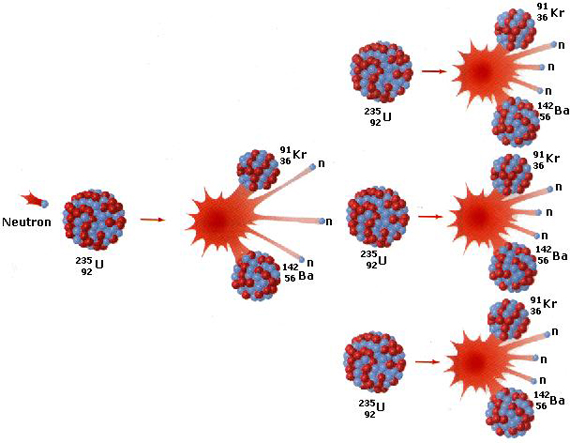
\includegraphics[width=0.95\textwidth]{ne585/fission.jpg}
                %\caption{}
            \end{figure}
        \end{column}

        \begin{column}{0.50\textwidth}
            \begin{figure}
                \centering
                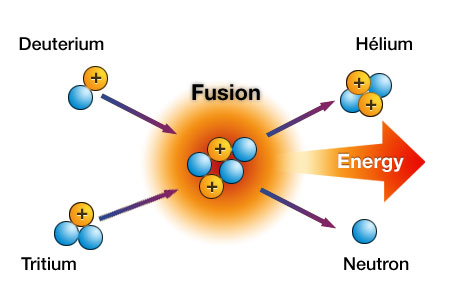
\includegraphics[width=0.95\textwidth]{ne585/fusion.jpg}
                %\caption{}
            \end{figure}
        \end{column}

    \end{columns}
\end{frame}


\begin{frame}{Determine the energy of a fusion neutron that is not at rest}
    \begin{equation}
        \LARGE 
        m = \frac{m_0}{\sqrt{1-(\frac{v^2}{c})^2}} \rightarrow E = m c^2
    \end{equation}
    
    \vspace*{\fill}

    \begin{enumerate}[series=outerlist,topsep=0pt,itemsep=21pt,leftmargin=*,label=(\arabic*)]
        \item[]With $v = 5.2 \times 10^7 \; m/s$, that is about $0.17c$; not negligible
        \item[]So we have to compute the not rest mass
        \item[]$m_0(n) = 1.674927211 \times 10^{-27} \; kg$
        \item[]Fusion neutron at that speed has $E = 14.5 \; MeV$
        \item[]For relativistic calculations use MeV
    \end{enumerate}
\end{frame}


\section{Atomic structure}


\addtocounter{framenumber}{-1}
\begin{frame}{The shell model describes how subatomic particles are arranged}
    \begin{columns}

        \begin{column}{0.50\textwidth}
            \begin{figure}
                \centering
                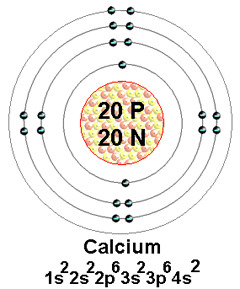
\includegraphics[width=0.75\textwidth]{ne585/calcium.jpg}
                %\caption{}
            \end{figure}
        \end{column}

        \begin{column}{0.50\textwidth}
            \begin{figure}
                \centering
                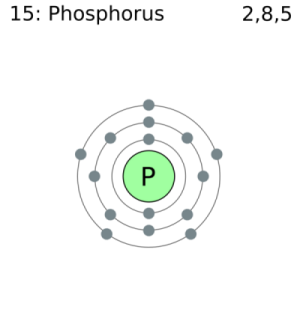
\includegraphics[width=0.95\textwidth]{ne585/phosphorus.jpg}
                %\caption{}
            \end{figure}
        \end{column}

    \end{columns}
\end{frame}


\begin{frame}{Notation}

    \vspace*{\fill}
    
    \centering
    \LARGE
    $^{A}_{Z}Q_{A-Z} = ^{235}_{92}U_{143}$

    \vspace*{\fill}

\end{frame}


\begin{frame}{}
    \begin{figure}
        \centering
        \href{https://ptable.com/}{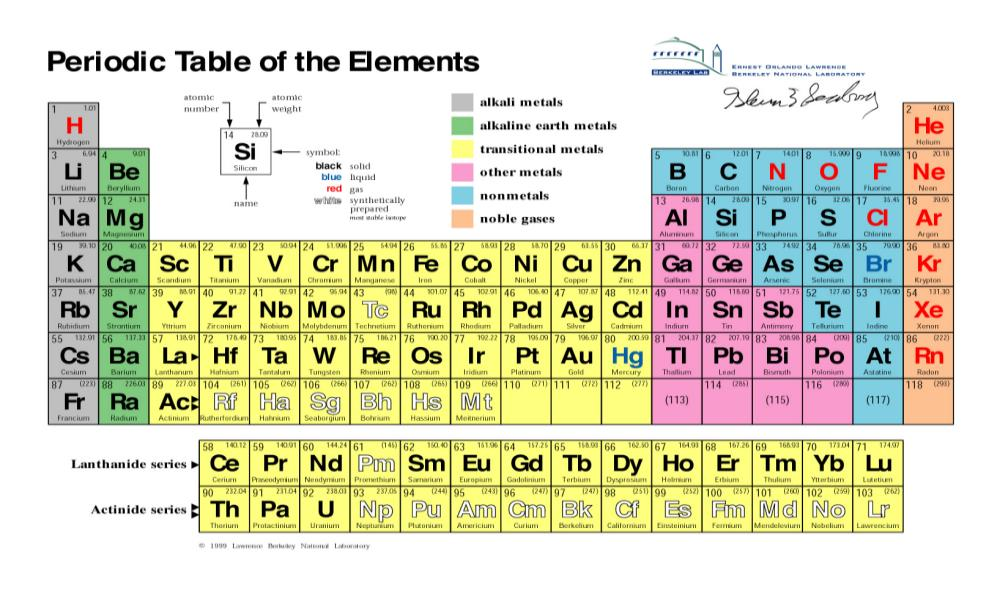
\includegraphics[width=0.95\textwidth]{ne585/periodic.table.jpg}}
%        \caption{}
    \end{figure}
\end{frame}


\section{Binding energy}


\addtocounter{framenumber}{-1}
\begin{frame}{There are four fundamental forces of interaction}
    \begin{enumerate}[series=outerlist,topsep=0pt,itemsep=21pt,leftmargin=*,label=(\arabic*)]
        \item[]Gravity -- Obvious
        \item[]\textit{Strong nuclear -- Holds the nucleus together}
        \item[]Electromagnetic -- Basically electrons \& magnetism
        \item[]Weak nuclear -- Changes the flavor of quarks
    \end{enumerate}
\end{frame}


\begin{frame}{To blow out a nucleus, a lot of energy is needed}
    \begin{enumerate}[series=outerlist,topsep=0pt,itemsep=21pt,leftmargin=*,label=(\arabic*)]
        \item[]Would it be constant or variable per nucleus?
        \item[]Why would you want to blow out the nucleus?
    \end{enumerate}

    \begin{equation}
        \LARGE
        \Delta m = (A-Z)m_n - Zm_p - M
    \end{equation}

    \begin{equation}
        \LARGE
        \Delta m(^{239}_{94}Pu) = 1759 \; MeV = 7.40 \; \frac{MeV}{nucleon}
    \end{equation}

    \vspace*{\fill}

    \begin{enumerate}[series=outerlist,topsep=0pt,itemsep=21pt,leftmargin=*,label=(\arabic*)]
        \item[]This energy corresponds to a velocity of 0.88c
        \item[]\LARGE $931.5 \; \frac{MeV}{amu}$
    \end{enumerate}
\end{frame}


\begin{frame}{Binding energy is used to compare atomic stability, reaction energy, probability of fission/fusion}
    \begin{figure}
        \centering
        \href{https://static.wixstatic.com/media/b89a36_1bd87fd3fe5c4d148c7a37c821c5187b~mv2.gif}{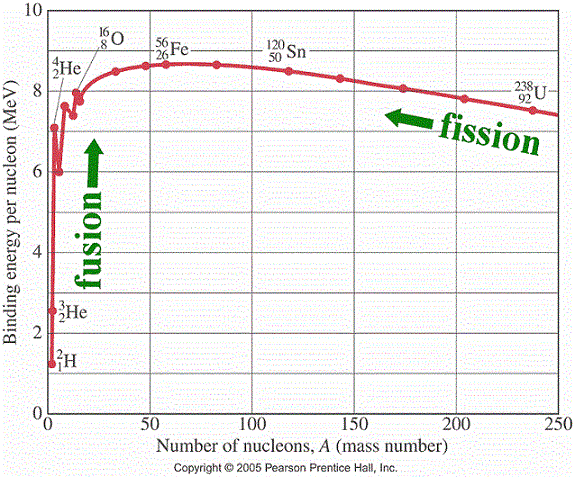
\includegraphics[width=0.55\textwidth]{ne585/binding.energy.jpg}}
%        \caption{}
    \end{figure}
\end{frame}


\begin{frame}{Light nuclei get more stable by fusion; heavy nuclei get more stable by fission}
    \begin{figure}
        \centering
        \href{http://ch302.cm.utexas.edu/images302/binding-energy.png}{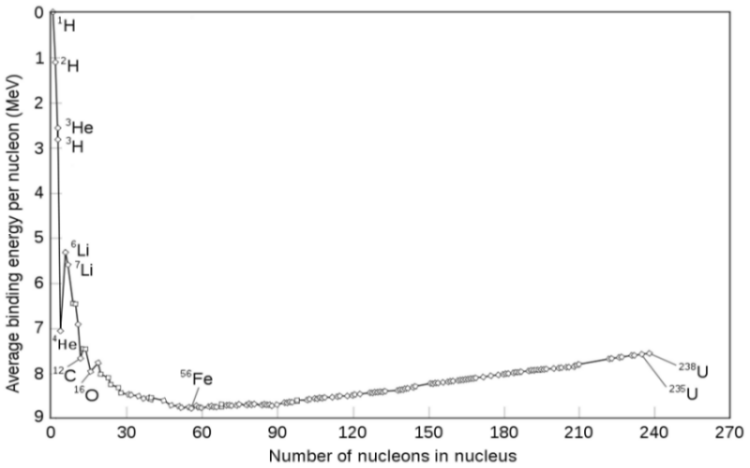
\includegraphics[width=0.75\textwidth]{ne585/binding.energy.invert.jpg}}
%        \caption{}
    \end{figure}
\end{frame}


\section{Q-value}


\addtocounter{framenumber}{-1}
\begin{frame}{The Q-value for a reaction indicates energy requirements}

    \begin{equation}
        \LARGE
        ^6_3Li \; (n,\alpha) \; ^3_1H
    \end{equation}

    \begin{equation}
        \LARGE
        ^6_3Li + ^1_0n \rightarrow ^4_2\alpha + ^3_1H
    \end{equation}

    \vspace*{\fill}

    \begin{enumerate}[series=outerlist,topsep=0pt,itemsep=15pt,leftmargin=*,label=(\arabic*)]
        \item Conservation of nucleons
        \item Conservation of charge
        \item Conservation of momentum
        \item Conservation of energy
    \end{enumerate}
\end{frame}


\begin{frame}{Compute the Q value for this reaction}

    \begin{equation}
        \LARGE
        ^6_3Li + ^1_0n \rightarrow ^4_2\alpha + ^3_1H
    \end{equation}

    \begin{equation}
        \LARGE
        Q = [(M_{Li} + M_n) - (M_{\alpha} + M_H)]c^2
    \end{equation}

    \begin{equation}
        \LARGE
        Q = 4.78 \; MeV
    \end{equation}

    \vspace*{\fill}

    \begin{enumerate}[series=outerlist,topsep=0pt,itemsep=21pt,leftmargin=*,label=(\arabic*)]
        \item[]\LARGE $Q > 0 \rightarrow \; ?$
        \item[]\LARGE $Q < 0 \rightarrow \; ?$
    \end{enumerate}
\end{frame}


\begin{frame}{What is the energy of fission from thorium and uranium fuel cycles?}

    \begin{equation}
        \LARGE
        ^1_0n + ^{235}_{92}U \rightarrow ^{92}_{36}Kr + ^{141}_{56}Ba + ^1_0n + ^1_0n + ^1_0n  
    \end{equation}

    \begin{equation}
        \LARGE
        ^1_0n + ^{233}_{92}U \rightarrow ^{92}_{36}Kr + ^{141}_{56}Ba + ^1_0n   
    \end{equation}

    \vspace*{\fill}

    \begin{enumerate}[series=outerlist,topsep=0pt,itemsep=21pt,leftmargin=*,label=(\arabic*)]
        \item[]For comparison, burning a carbon atom releases 4 eV
    \end{enumerate}
\end{frame}


\section{Radioactivity}


\addtocounter{framenumber}{-1}
\begin{frame}{Scientists in late 1800s made discoveries which would change the course of science, medicine, and history in the 20th Century}
    \begin{figure}
        \centering
        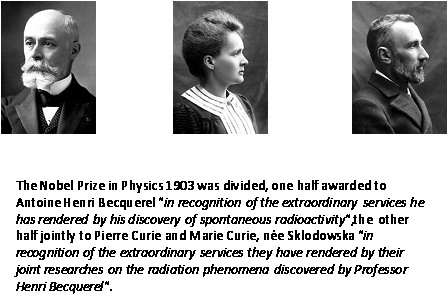
\includegraphics[width=0.75\textwidth]{ne585/nobel.jpg}
%        \caption{}
    \end{figure}
\end{frame}


\begin{frame}{Radiation is energy as particles or electromagnetic waves, like sunshine}
    \begin{figure}
        \centering
        \href{https://www.researchgate.net/profile/Ngai_Chan/publication/277996216/figure/fig5/AS:336497640263680@1457238697222/The-electromagnetic-spectrum-for-different-frequency-bands-and-the-corresponding.jpg}{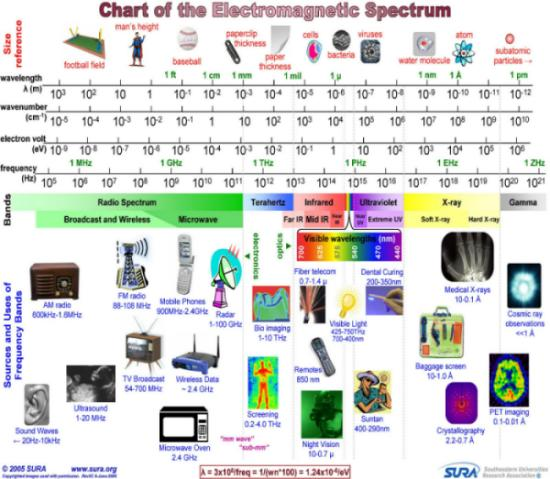
\includegraphics[width=0.55\textwidth]{ne585/waves.jpg}}
%        \caption{}
    \end{figure}
\end{frame}


\begin{frame}{Radiation is energy as particles or electromagnetic waves}
    \begin{columns}

        \begin{column}{0.50\textwidth}
            \begin{figure}
                \centering
                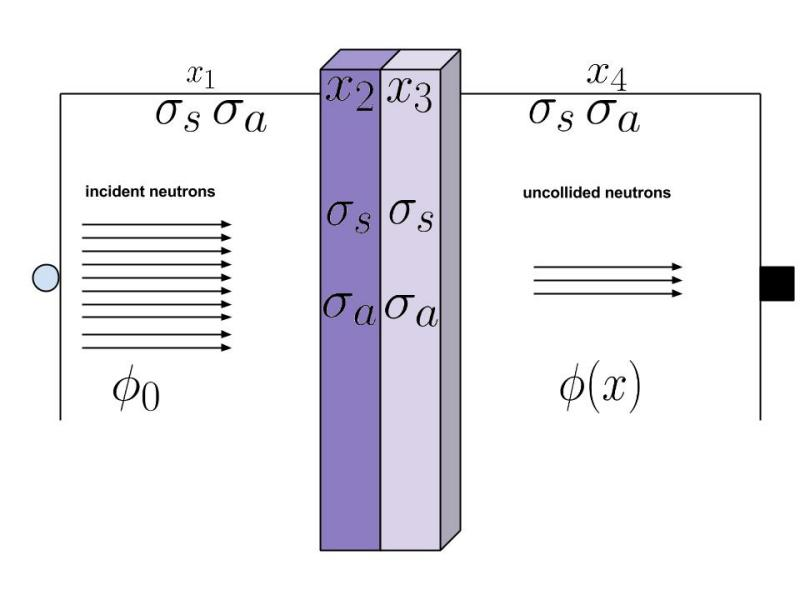
\includegraphics[width=0.75\textwidth]{ne585/shielding.jpg}
                %\caption{}
            \end{figure}
        \end{column}

        \begin{column}{0.50\textwidth}
            \begin{figure}
                \centering
                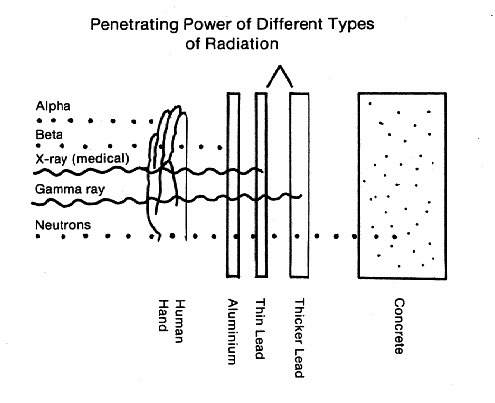
\includegraphics[width=0.95\textwidth]{ne585/shielding2.jpg}
                %\caption{}
            \end{figure}
        \end{column}

    \end{columns}
\end{frame}


\begin{frame}{Radiation is energy as particles or electromagnetic waves}
    Charged particles are --
    \begin{itemize}[series=outerlist,topsep=0pt,itemsep=5pt]
        \item protons (+)
        \item alpha (++)
        \item beta (+/-)
        \item heavy ions (varying)
        \item U,Pu (3+,4+,5+,6+)
    \end{itemize}

    \vspace*{\fill}

    \begin{enumerate}[series=outerlist,topsep=0pt,itemsep=21pt,leftmargin=*,label=(\arabic*)]
        \item[]Neutrons have no charge, but are also ionizing
        \item[]Ionizing rays are x-rays, g-rays, cosmic rays
    \end{enumerate}
\end{frame}


\begin{frame}{Ernest Rutherford discovered the three main kinds of radioactive decay (Chemistry Nobel 08)}
    \begin{figure}
        \centering
        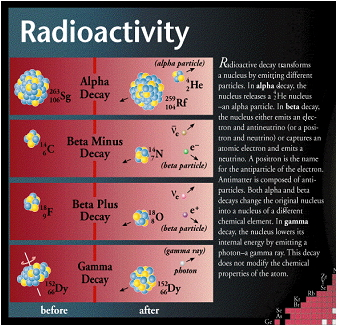
\includegraphics[width=0.45\textwidth]{ne585/radioactivity.jpg}
%        \caption{}
    \end{figure}
\end{frame}


\begin{frame}{Alpha particle decay is the ejection of a helium atom from a heavy nucleus}

    \begin{equation}
        \LARGE
        ^{238}_{92}U \rightarrow ^{234}_{90}Th + ^{4}_{2}\alpha  
    \end{equation}

    \begin{equation}
        \LARGE
        Q = 4.268 \; MeV
    \end{equation}

    \vspace*{\fill}

    \begin{enumerate}[series=outerlist,topsep=0pt,itemsep=21pt,leftmargin=*,label=(\arabic*)]
        \item[]Sometimes nucleus decays to excited state and then emits a gamma ray (for any kind of radiation)
        \item[]Discrete energy spectrum
        \item[]Some \% decay at certain energy
    \end{enumerate}
\end{frame}


\begin{frame}{}
    \begin{figure}
        \centering
        \href{https://courses.ecampus.oregonstate.edu/ne581/three/images/chart32.gif}{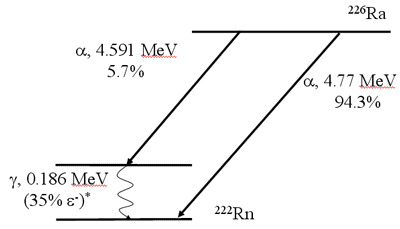
\includegraphics[width=0.55\textwidth]{ne585/alpha.con.jpg}}
%        \caption{}
    \end{figure}
\end{frame}


\begin{frame}{$\beta^-$ particle decay occurs for unstable nuclei with excessive neutrons}

    \begin{equation}
        \LARGE
        ^{19}_{8}O \rightarrow ^{19}_{9}F + \beta^{-} + \overline{\nu} 
    \end{equation}

    \vspace*{\fill}

    \begin{enumerate}[series=outerlist,topsep=0pt,itemsep=21pt,leftmargin=*,label=(\arabic*)]
        \item[]The neutron is converted to a proton and a beta negative (electron) and anti-neutrino (momentum) are ejected
        \item[]Sometimes nucleus decays to excited state and then emits a gamma ray (for any kind of radiation)
    \end{enumerate}
\end{frame}


\begin{frame}{}
    \begin{figure}
        \centering
        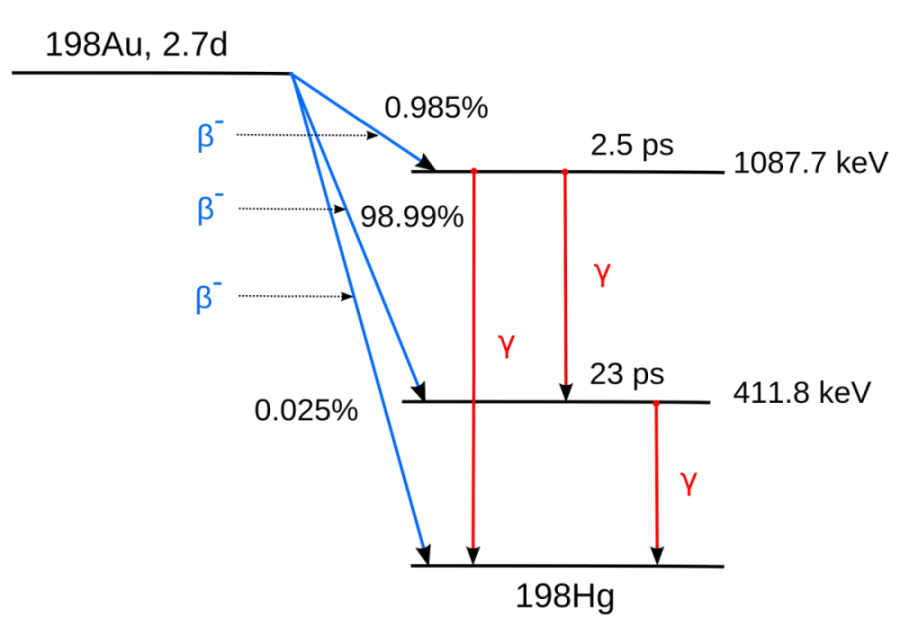
\includegraphics[width=0.55\textwidth]{ne585/beta.con.jpg}
%        \caption{}
    \end{figure}
\end{frame}


\begin{frame}{$\beta^+$ particle decay occurs for unstable nuclei with deficient neutrons}

    \begin{equation}
        \LARGE
        ^{11}_{6}C \rightarrow ^{11}_{5}B + \beta^{+} + \nu 
    \end{equation}

    \vspace*{\fill}

    \begin{enumerate}[series=outerlist,topsep=0pt,itemsep=21pt,leftmargin=*,label=(\arabic*)]
        \item[]The proton is converted to a neutron and a beta positive (positron) and neutrino (momentum) are ejected
        \item[]Sometimes nucleus decays to excited state and then emits a gamma ray (for any kind of radiation)
    \end{enumerate}
\end{frame}


\begin{frame}{}
    \begin{figure}
        \centering
        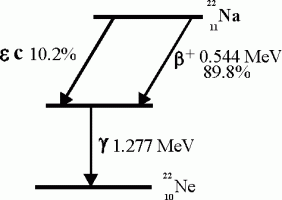
\includegraphics[width=0.55\textwidth]{ne585/betaplus.con.jpg}
%        \caption{}
    \end{figure}
\end{frame}


\begin{frame}{In both forms of beta decay, the energies are exhibited by a continuous energy spectrum}
    \begin{figure}
        \centering
        \href{http://images.slideplayer.com/17/5357960/slides/slide_24.jpg}{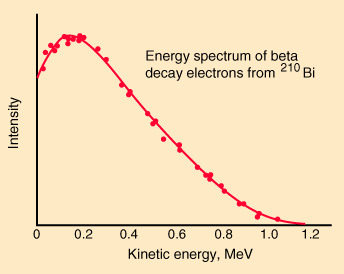
\includegraphics[width=0.30\textwidth]{ne585/beta.spectrum.jpg}}
%        \caption{}
    \end{figure}

    \vspace*{\fill}

    \begin{equation}
        \LARGE
        \overline{E}(\beta^-)=0.3E_{MAX}
    \end{equation}

    \begin{equation}
        \LARGE
        \overline{E}(\beta^+)=0.4E_{MAX}
    \end{equation}
\end{frame}


\begin{frame}{Electron capture also occurs for unstable nuclei with deficient neutrons}

    \begin{equation}
        \LARGE
        ^{22}_{11}Na \rightarrow \epsilon^- + ^{22}_{10}Ne + \nu 
    \end{equation}

    \vspace*{\fill}

    \begin{enumerate}[series=outerlist,topsep=0pt,itemsep=21pt,leftmargin=*,label=(\arabic*)]
        \item[]The K shell electron (not free) is absorbed by the nucleus to convert the proton to a neutron
        \item[]Sometimes nucleus decays to excited state and then emits a gamma ray (for any kind of radiation)
    \end{enumerate}
\end{frame}


\begin{frame}{}
    \begin{figure}
        \centering
        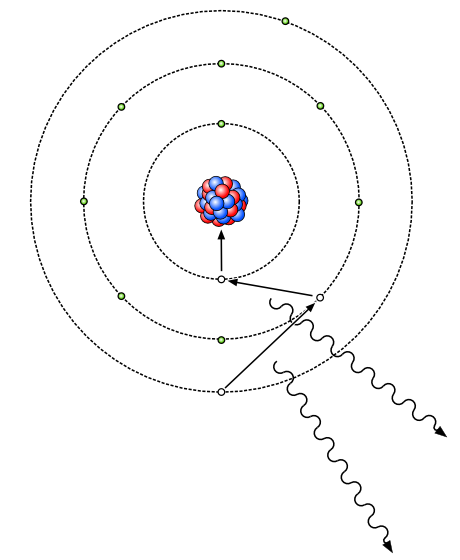
\includegraphics[width=0.45\textwidth]{ne585/ec.shell.jpg}
%        \caption{}
    \end{figure}
\end{frame}


\begin{frame}{Electron capture and $\beta^+$ are competing processes}

    \begin{equation}
        \LARGE
        ^{22}_{11}Na \rightarrow \epsilon^- + ^{22}_{10}Ne + \nu 
    \end{equation}

    \begin{equation}
        \LARGE
        ^{22}_{11}Na \rightarrow ^{22}_{10}Ne + \beta^{+} + \nu 
    \end{equation}

    \begin{equation}
        \LARGE
        Q = 2.842 \; MeV
    \end{equation}

    \vspace*{\fill}

    \begin{enumerate}[series=outerlist,topsep=0pt,itemsep=21pt,leftmargin=*,label=(\arabic*)]
        \item[]$Q > 1.022 \; MeV$ positron favored
        \item[]$Q < 1.022 \; MeV$ electron capture favored
        \item[]Why?
    \end{enumerate}
\end{frame}


\begin{frame}{$\gamma$-ray emission is not a decay mode, but superfast de-excitation of the nucleus}
    \begin{enumerate}[series=outerlist,topsep=0pt,itemsep=21pt,leftmargin=*,label=(\arabic*)]
        \item[]Interactions of gamma rays with matter is a very important branch of nuclear physics
    \end{enumerate}
\end{frame}


\section{Chart of the nuclides}


\addtocounter{framenumber}{-1}
\begin{frame}{}
    \begin{figure}
        \centering
        \href{https://www.nndc.bnl.gov/chart/}{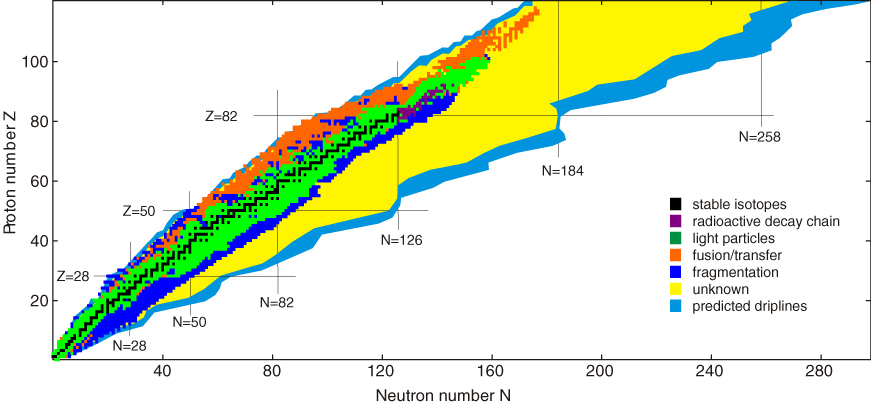
\includegraphics[width=0.90\textwidth]{ne585/chart.jpg}}
%        \caption{}
    \end{figure}
\end{frame}


\begin{frame}{}
    \begin{figure}
        \centering
        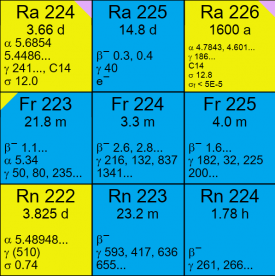
\includegraphics[width=0.50\textwidth]{ne585/chart.example.jpg}
%        \caption{}
    \end{figure}
\end{frame}


\section{Decay chains}


\addtocounter{framenumber}{-1}
\begin{frame}{}
    \begin{figure}
        \centering
        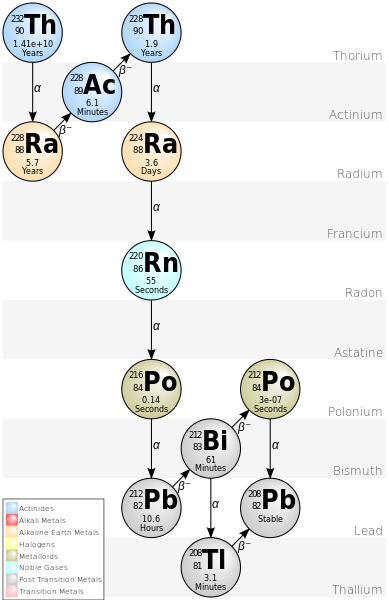
\includegraphics[width=0.30\textwidth]{ne585/th232.chain.jpg}
%        \caption{}
    \end{figure}
\end{frame}


\begin{frame}{}
    \begin{figure}
        \centering
        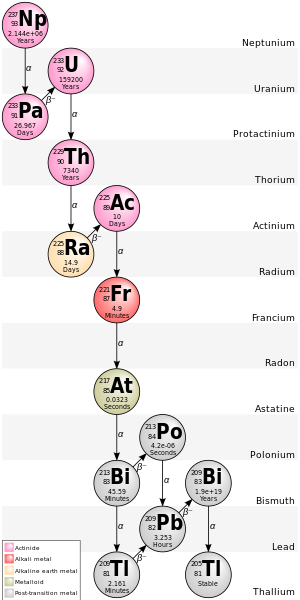
\includegraphics[width=0.30\textwidth]{ne585/np237.chain.jpg}
%        \caption{}
    \end{figure}
\end{frame}


\begin{frame}{}
    \begin{figure}
        \centering
        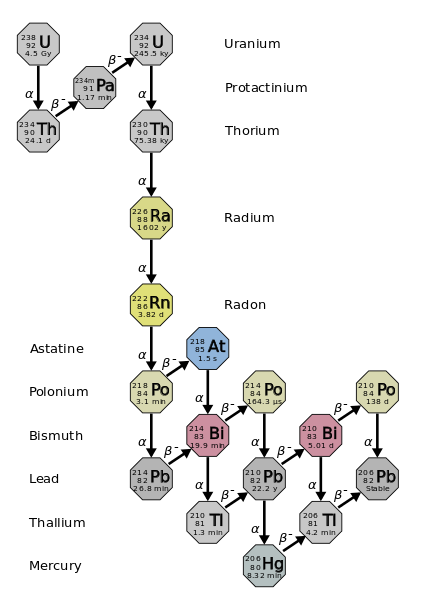
\includegraphics[width=0.30\textwidth]{ne585/u238.chain.jpg}
%        \caption{}
    \end{figure}
\end{frame}


\begin{frame}{}
    \begin{figure}
        \centering
        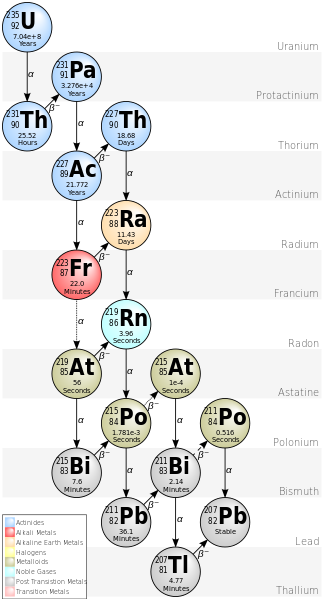
\includegraphics[width=0.30\textwidth]{ne585/u235.chain.jpg}
%        \caption{}
    \end{figure}
\end{frame}


\section{Half life}


\addtocounter{framenumber}{-1}
\begin{frame}{A radioactive isotope decays with a unique characteristic time}
    \begin{enumerate}[series=outerlist,topsep=0pt,itemsep=21pt,leftmargin=*,label=(\arabic*)]
        \item[]Decay is stochastic, characterized by Poisson distribution
        \item[]So the decay of any one radionuclide cannot be predicted
        \item[]The probability per time that a nucleus will decay is a constant
    \end{enumerate}
\end{frame}


\begin{frame}{Decay is described by a \href{https://stattrek.com/probability-distributions/poisson.aspx}{Poisson process}}
    \begin{enumerate}[series=outerlist,topsep=0pt,itemsep=21pt,leftmargin=*,label=(\arabic*)]
        \item[]Occurrences are randomly distributed in time
        \item[]What is the `occurrence' here?
        \item[]Homogeneous, long term decay rate is constant
    \end{enumerate}

    \vspace*{\fill}

    \begin{equation}
        \LARGE
        \mu \equiv \lambda \Delta t
    \end{equation}

    \begin{equation}
        \LARGE
        P(n) = e^{-\mu} \cdot \frac{\mu^n}{n!}
    \end{equation}

    \vspace*{\fill}

    \begin{enumerate}[series=outerlist,topsep=0pt,itemsep=21pt,leftmargin=*,label=(\arabic*)]
        \item[]What is the \href{https://uidaho.pressbooks.pub/riskassessment/chapter/statistical-moments/}{expected value and variance} of the distribution?
    \end{enumerate}
\end{frame}


\begin{frame}{A radioactive isotope decays with a unique characteristic time}
    \begin{enumerate}[series=outerlist,topsep=0pt,itemsep=21pt,leftmargin=*,label=(\arabic*)]
        \item[]$n(t)$ atoms at $t$ have decayed in $dt$
    \end{enumerate}

    \vspace*{\fill}

    \begin{equation}
        \LARGE
        \lambda n(t) dt
    \end{equation}

    \vspace*{\fill}

    \begin{enumerate}[series=outerlist,topsep=0pt,itemsep=21pt,leftmargin=*,label=(\arabic*)]
        \item[]The number of atoms that decay on average in the interval $t,(t+dt)$ can be expressed as --
    \end{enumerate}

    \vspace*{\fill}

    \begin{equation}
        \LARGE
        -dn(t)=\lambda n(t) dt
    \end{equation}

    \vspace*{\fill}

    \begin{enumerate}[series=outerlist,topsep=0pt,itemsep=21pt,leftmargin=*,label=(\arabic*)]
        \item[]You should be able to solve this for $n(0)=n_0$
    \end{enumerate}
\end{frame}


\begin{frame}{Radionuclides are characterized by half life}

    \begin{equation}
        \LARGE
        t_{\frac{1}{2}}=\frac{ln 2}{\lambda}
    \end{equation}

    \vspace*{\fill}

    \begin{enumerate}[series=outerlist,topsep=0pt,itemsep=21pt,leftmargin=*,label=(\arabic*)]
        \item[]Half life can be derived from the decay law
    \end{enumerate}
\end{frame}


\begin{frame}{A radionuclide is `negligible' after 10 half-lives have elapsed}

    \begin{figure}
        \centering
        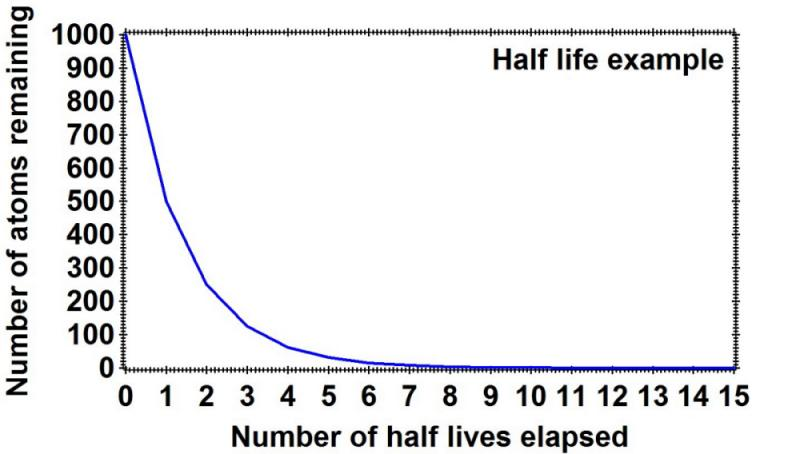
\includegraphics[width=0.75\textwidth]{ne585/half.life.example.jpg}
%        \caption{}
    \end{figure}

    \vspace*{\fill}

    \begin{enumerate}[series=outerlist,topsep=0pt,itemsep=21pt,leftmargin=*,label=(\arabic*)]
        \item[]Why would this be important?
    \end{enumerate}
\end{frame}


\begin{frame}{How was half-life discovered?}
    \begin{enumerate}[series=outerlist,topsep=0pt,itemsep=21pt,leftmargin=*,label=(\arabic*)]
        \item[]Rutherford discovered alpha and beta particle decay
        \item[]In the course of, he noticed that there was a characteristic time
        \item[]Basically observed decay time was the same for each atom
        \item[]Experiments with thorium led to the discovery of radon
        \item[]Then observing the radon gas led to the decay/half-life (65 s)
    \end{enumerate}
\end{frame}


\begin{frame}{}
    \begin{figure}
        \centering
        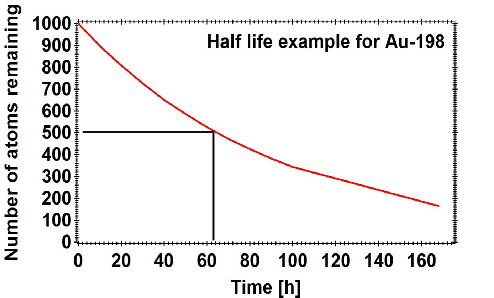
\includegraphics[width=0.75\textwidth]{ne585/au198.linear.jpg}
%        \caption{}
    \end{figure}
\end{frame}


\begin{frame}{Engineers like straight lines}
    \begin{figure}
        \centering
        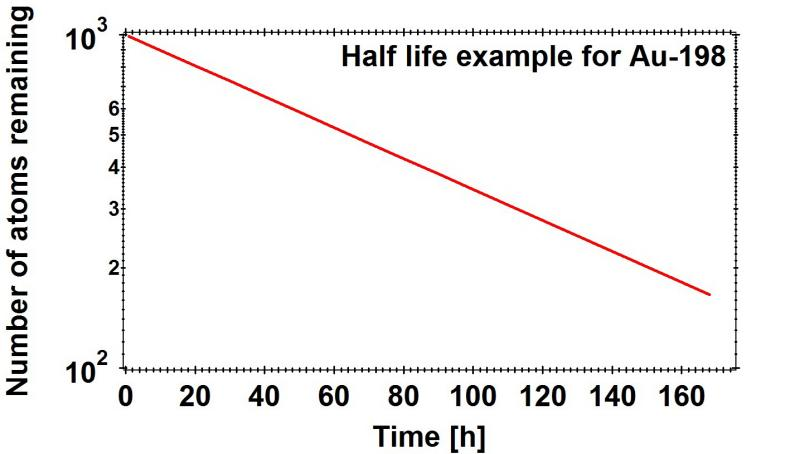
\includegraphics[width=0.75\textwidth]{ne585/au198.log.jpg}
%        \caption{}
    \end{figure}

    \vspace*{\fill}

    \begin{enumerate}[series=outerlist,topsep=0pt,itemsep=21pt,leftmargin=*,label=(\arabic*)]
        \item[]Slope of the line is the decay constant
    \end{enumerate}
\end{frame}


\begin{frame}[plain]{}
    \begin{figure}
        \centering
        \includegraphics[width=0.45\textwidth]{ne585/1-final.jpg}
%        \caption{}
    \end{figure}
\end{frame}


%%%%%%%
%\begin{frame}{}
%    \begin{columns}
%
%        \begin{column}{0.50\textwidth}
%            \begin{enumerate}[series=outerlist,topsep=0pt,itemsep=21pt,leftmargin=*,label=(\arabic*)]
%                \item[]
%                \item[]
%            \end{enumerate}
%        \end{column}
%
%        \begin{column}{0.50\textwidth}
%            \begin{enumerate}[series=outerlist,topsep=0pt,itemsep=21pt,leftmargin=*,label=(\arabic*)]
%                \item[]
%                \item[]
%            \end{enumerate}
%        \end{column}
%
%    \end{columns}
%\end{frame}

%    \begin{figure}
%        \centering
%        \includegraphics[width=0.75\textwidth]{wsc.png}
%        \caption{\acs{wsc}}
%    \end{figure}


%\begin{frame}{References}
%    \bibliographystyle{nsf}
%    \footnotesize
%    \bibliography{references}
%\end{frame}
%%%%%%%


\end{document}
